\chapter{Testy i ocena aplikacji}

\section{Testy jednostkowe i instrumentalne aplikacji mobilnej (Dorota Tomczak)}
\par Dla aplikacji mobilnej napisano 23 testy jednostkowe oraz 9 instrumentalnych, które obejmują klasy i metody komponentów służących do logowania, rejestracji oraz przekierowania po starcie aplikacji. Testy jednostkowe, czyli takie które weryfikują poprawność realizacji pojedynczych funkcjonalności aplikacji, zostały zbudowane w oparciu o następujące zależności: \textit{JUnit 4} \cite{JUnit}, \textit{JUnitParams} \cite{JUnitParams} do tworzenia testów parametryzowanych oraz bibliotekę \textit{MockK} \cite{MockK} służącą do tworzenia atrap obiektów (ang. mock object) w języku Kotlin. Testy te służą do weryfikacji działania metod zdefiniowanych w prezenterach, z tego względu przed startem każdego z nich odpowiedni prezenter nie jest atrapą, ale jest inicjalizowany w sposób, który umożliwia jego „szpiegowanie”. Aby zasymulować asynchroniczną komunikację sieciową pomiędzy aplikacją a serwerem, która odbywa się poprzez zastosowanie biblioteki \textit{RxJava} \cite{RxJava}, stworzono klasę pomocniczą \textit{RxImmediateJavaSchedulerRule}, która ustawia wszystkie metody, rozpoczynające nowe wątki, aby korzystały zamiast tego z wątku obecnego.
\par Testy instrumentalne, czyli takie które działają na emulatorze lub na fizycznym urządzeniu mobilnym, zostały zrealizowane dla dwóch aktywności – \textit{SignInActivity} oraz \textit{SignUpActivity} i testują, czy na ekranie wyświetlają się prawidłowe informacje, czy akcje użytkownika wywołują odpowiednie metody oraz czy aplikacja reaguje na nie w odpowiedni sposób. Wykorzystują wiele zależności, w tym między innymi \textit{Espresso} \cite{Espresso} i \textit{MockK-Android} \cite{MockK-Android}. W klasach testowych tworzone są role aktywności (\textit{activityScenarioRole}), na których następnie można wywoływać określone akcje np. wciśnięcie przycisku, czy wpisanie tekstu w polu do tego przeznaczonym (rys.~\ref{fig:instrumentationTest}).

\begin{figure}[h]
\centering
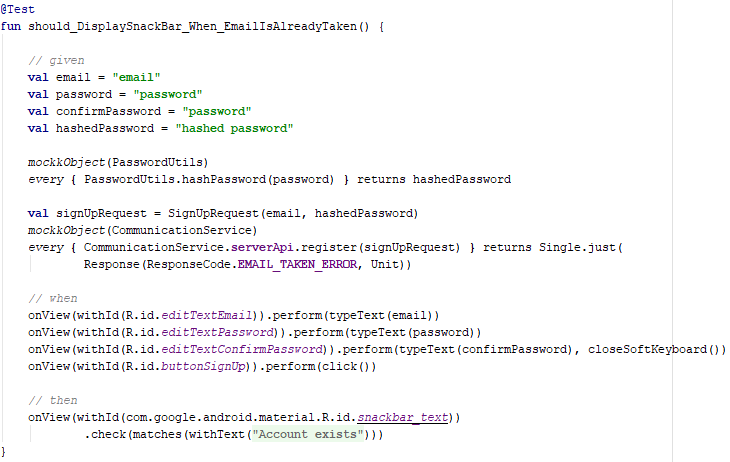
\includegraphics[width=\linewidth]{instrumentationTest}
\caption{Przykładowy test instrumentalny.}
\label{fig:instrumentationTest}
\end{figure}

\par Wszystkie testy, zarówno instrumentalne jak i jednostkowe zostały podzielone na trzy segmenty:
\begin{itemize}
\item \textit{given} -- definicja danych wejściowych oraz symulowanie wywołań metod i tworzenie atrap obiektów,
\item \textit{when} -- wywołanie testowanej metody lub wykonanie akcji,
\item \textit{then} -- weryfikacja otrzymanych rezultatów po wywołaniu metody lub wykonaniu akcji.
\end{itemize}
Do nazewnictwa testów przyjęto następującą konwencję: co powinno się stać, gdy zostaną spełnione określone warunki. Przykładowo \textit{Should display snackBar with info message when given password in SignUp is incorrect}, co w tłumaczeniu oznacza \textit{Powinien się wyświetlić snackBar z komunikatem informacyjnym, gdy hasło podane w SignUp jest nieprawidłowe}.

\FloatBarrier

\section{Testy dostępu do bazy danych (Magdalena Solecka)}
\par Napisano 73 testy dostępu do bazy danych przy użyciu bibliotek JUnit \cite{JUnit} oraz MockK \cite{MockK}. Przyjęto założenie, że rekordy o indeksie 0 będą danymi stałymi wykorzystywanymi do testowania operacji odczytu (ang. select) oraz aktualizacji (ang. update). Problematyczne okazały się jednak funkcje testujące usuwanie i dodawanie danych do bazy (rys.~\ref{fig:dbTests}). W tych przypadkach należało wykonać obie te operacje: najpierw wstawienie wartości, a następnie jej usunięcie ze sprawdzeniem poprawności za pomocą polecenia Assert.assertTrue jako polecenie następne po tym testowanym. Oznacza to jednak, że test nie jest w pełni testem jednostkowym, gdyż wykonuje więcej niż jedną operację. Dla każdej testowanej funkcji rozpatrzono wszystkie przypadki poprawnego jej wykonania, np. dla funkcji pobierającej rekord z bazy na podstawie id (get(id:Int)) było to zwrócenie obiektu typu User jeśli podane w bazie istniał wiersz z zadanym id oraz zwrócenie wartości null przy podaniu numeru id, które nie znajduje się w bazie. 

\begin{figure}[h]
\centering
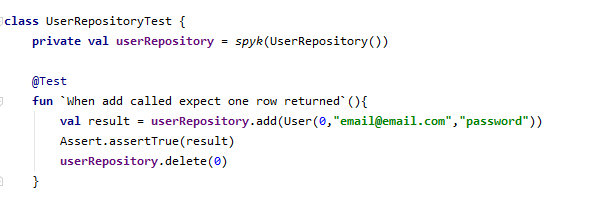
\includegraphics[width=\linewidth]{dbTests}
\caption{Test operacji dodawania obiektu User do bazy danych.}
\label{fig:dbTests}
\end{figure}
\FloatBarrier

\section{Ocena aplikacji (Magdalena Solecka)}
\par Wszystkie wymagania funkcjonalne o priorytecie wysokim zdefiniowane w specyfikacji 
wymagań systemowych zostały zrealizowane. Jest to jednoznaczne ze spełnieniem przyjętego 
na etapie planowania projektu kryterium akceptacyjnego. 

\par Dodatkowymi zaletami aplikacji są spełnione częściowo wymagania wiarygodności. Spośród sześciu wymagań o priorytecie średnim zostały zrealizowane trzy: skanowanie biletów, przeglądanie ofert zakwaterowania/hoteli i oznaczanie elementu planu dnia jako ukończony. Zrealizowano również jedno z dwóch zdefiniowanych wymagań funkcjonalnych o priorytecie niskim: udostępnienie elementu planu dnia w medium społecznościowym. Zgodnie z wymaganiami 
wiarygodności nie wymaga się od użytkownika podawania danych wrażliwych (ochrona danych 
użytkownika: priorytet wysoki), a hasła przechowywane są w postaci zaszyfrowanej 
(szyfrowanie przesyłanych danych priorytet średni). Nie można ocenić realizacji wymagań 
wydajnościowych ze względu na brak jakichkolwiek testów tego rodzaju. Z wymagań w 
zakresie elastyczności o priorytecie wysokim spełniono możliwość uruchomienia aplikacji 
w systemie Android. Program przetestowano m.in. w systemie Android wersji 9 Pie (API 
28).